\aula{03b}{03}{setembro}{2026}

\begin{resposta}
    \begin{enumerate}[start=7]
        \item Compatibilização dos momentos fletores

        \begin{figure}[H]
    \centering
    \begin{tikzpicture}[
        scale=1.5,
        retangulo/.style={draw=gray!80!black, thick},
        rotuloLetra/.style={font=\footnotesize, blue!80!black},
        eixo/.style={->, >=stealth, thick, black},
        corte/.style={draw=black, dash dot, thick},
        setaCorte/.style={->, >=stealth, thick, black}
    ]

        % --- Definição dos Parâmetros de Dimensão ---
        \def\wCentro{3.2}       % Largura dos retângulos centrais (L1 e L3)
        \def\hCima{2.0}         % Altura do retângulo superior (L1)
        \def\hBaixo{2.2}        % Altura do retângulo inferior (L3)
        
        \def\wDir{2.2}          % Largura do retângulo da direita (L2)
        \def\hDir{\hCima + \hBaixo} % Altura total da laje L2
        
        \def\wEsq{1.6}          % Largura do retângulo da esquerda (L4)
        \def\hEsq{\hBaixo}      % Altura da laje L4

        % --- Coordenadas ---
        \coordinate (A2) at (0, 0);
        \coordinate (B2) at (\wCentro, 0);
        \coordinate (C2) at (\wCentro, \hBaixo);
        \coordinate (D2) at (0, \hBaixo);

        \coordinate (A1) at (0, \hBaixo);
        \coordinate (B1) at (\wCentro, \hBaixo);
        \coordinate (C1) at (\wCentro, \hBaixo + \hCima);
        \coordinate (D1) at (0, \hBaixo + \hCima);

        \coordinate (A3) at (\wCentro, 0);
        \coordinate (B3) at (\wCentro + \wDir, 0);
        \coordinate (C3) at (\wCentro + \wDir, \hDir);
        \coordinate (D3) at (\wCentro, \hDir);

        \coordinate (A4) at (-\wEsq, 0);
        \coordinate (B4) at (0, 0);
        \coordinate (C4) at (0, \hEsq);
        \coordinate (D4) at (-\wEsq, \hEsq);

        % --- Desenho dos Retângulos ---
        \draw[retangulo] (A1) rectangle (C1); % L1
        \draw[retangulo] (A2) rectangle (C2); % L3
        \draw[retangulo] (A3) rectangle (C3); % L2
        \draw[retangulo] (A4) rectangle (C4); % L4

        % --- EIXOS LOCALIZADOS COM NÚMERO NO CENTRO DE CADA EIXO ---
        % L1 (Topo)
        \coordinate (CL1) at ($(A1)!0.4!(C1)$);
        \draw[eixo] (CL1) -- ($(CL1)+(0.55,0)$) 
            node[midway, below=2pt, blue!80!black, fill=white, inner sep=1pt, font=\footnotesize] {0,76} 
            node[right=-2pt, font=\small] {$y$};
        \draw[eixo] (CL1) -- ($(CL1)+(0,0.55)$) 
            node[midway, left=2pt, blue!80!black, fill=white, inner sep=1pt, font=\footnotesize] {2,43} 
            node[above=-2pt, font=\small] {$x$};

        % L2 (Direita)
        \coordinate (CL2) at ($(A3)!0.5!(C3)$);
        \draw[eixo] (CL2) -- ($(CL2)+(0.55,0)$) 
            node[midway, below=2pt, blue!80!gray, fill=white, inner sep=1pt, font=\footnotesize] {7,80} 
            node[right=-2pt, font=\small] {$x$};
        \draw[eixo] (CL2) -- ($(CL2)+(0,0.55)$) 
            node[midway, left=2pt, blue!80!gray, fill=white, inner sep=1pt, font=\footnotesize] {2,24} 
            node[above=-2pt, font=\small] {$y$};

        % L4 (Baixo)
        \coordinate (CL3) at ($(A2)!0.4!(C2)$);
        \draw[eixo] (CL3) -- ($(CL3)+(0.55,0)$) 
            node[midway, below=2pt, blue!80!gray, fill=white, inner sep=1pt, font=\footnotesize] {5,36} 
            node[right=-2pt, font=\small] {$x$};
        \draw[eixo] (CL3) -- ($(CL3)+(0,0.55)$) 
            node[midway, left=2pt, blue!80!gray, fill=white, inner sep=1pt, font=\footnotesize] {4,04} 
            node[above=-2pt, font=\small] {$y$};

        % L3 (Esquerda)
        \coordinate (CL4) at ($(A4)!0.4!(C4)$);
        \draw[eixo] (CL4) -- ($(CL4)+(0.55,0)$) 
            node[midway, below=2pt, blue!80!gray, fill=white, inner sep=1pt, font=\footnotesize] {-1,10} 
            node[right=-2pt, font=\small] {$x$};
        \draw[eixo] (CL4) -- ($(CL4)+(0,0.55)$) 
            node[midway, left=2pt, blue!80!gray, fill=white, inner sep=1pt, font=\footnotesize] {0,07} 
            node[above=-2pt, font=\small] {$y$};

        % --- LINHAS DE CORTE A, B e C ---
        % Corte A: passa na L1 e L2
        \draw[corte] (-0.4, 2.85) -- (\wCentro + \wDir + 0.4, 2.85);
        \draw[setaCorte] (-0.4, 2.85) -- (-0.4, 3.15) node[above, font=\small\bfseries] {A};
        \draw[setaCorte] (\wCentro + \wDir + 0.4, 2.85) -- (\wCentro + \wDir + 0.4, 3.15) node[above, font=\small\bfseries] {A};

        % Corte B: da L3 a L2 (passando por L4)
        \draw[corte] (-\wEsq - 0.4, 0.5) -- (\wCentro + \wDir + 0.4, 0.5);
        \draw[setaCorte] (-\wEsq - 0.4, 0.5) -- (-\wEsq - 0.4, 0.8) node[above, font=\small\bfseries] {B};
        \draw[setaCorte] (\wCentro + \wDir + 0.4, 0.5) -- (\wCentro + \wDir + 0.4, 0.8) node[above, font=\small\bfseries] {B};

        % Corte C: de L1 a L4
        \draw[corte] (0.6, \hDir + 0.4) -- (0.6, -0.4);
        \draw[setaCorte] (0.6, \hDir + 0.4) -- (0.9, \hDir + 0.4) node[right, font=\small\bfseries] {C};
        \draw[setaCorte] (0.6, -0.4) -- (0.9, -0.4) node[right, font=\small\bfseries] {C};

        % --- Rótulos de Esforço Cortante nas Arestas ---
        % L1 (Topo)
        %\node[below, rotuloLetra] at ($(D1)!0.5!(C1)$) {$V_x$}; 
        %\node[right, rotuloLetra] at ($(D1)!0.5!(A1)$) {$V_y$}; 
        \node[above, rotuloLetra] at ($(A1)!0.5!(B1)$) {$5,12$};
        \node[left, rotuloLetra]  at ($(B1)!0.5!(C1)$) {$3,61$}; 

        % L3 (Baixo)
        \node[below, rotuloLetra] at ($(A1)!0.5!(B1)$) {$11,54$};
        \node[right, rotuloLetra] at ($(D2)!0.5!(A2)$) {$0$}; 
        %\node[above, rotuloLetra] at ($(A2)!0.5!(B2)$) {$V_y$};
        \node[left, rotuloLetra]  at ($(B2)!0.5!(C2)$) {$12,89$};  
        
        % L2 (Direita)
        \node[right, rotuloLetra] at ($(B1)!0.5!(C2)$) {$16,04$}; 
        %\node[below, rotuloLetra] at ($(D3)!0.5!(C3)$) {$V_y$}; 
        %\node[left= rotuloLetra]  at ($(C3)!0.5!(B3)$) {$V_x$}; 
        %\node[above, rotuloLetra] at ($(A3)!0.5!(B3)$) {$V_y$}; 

        % L4 (Esquerda)
        \node[left, rotuloLetra]  at ($(D2)!0.5!(A2)$) {$13,59$}; 
        %\node[below, rotuloLetra] at ($(D4)!0.5!(C4)$) {$V_y$}; 
        %\node[above, rotuloLetra] at ($(A4)!0.5!(B4)$) {$V_y$}; 
        \node[left, rotuloLetra]  at ($(D4)!0.5!(A4)$) {$0,98$}; 
        \draw[retangulo,white,dashed] (D4) rectangle (A4);
        
        \node[below, right=50pt] at ($(A3)!0.5!(B3)$) {$kN m/m$}; 

    \end{tikzpicture}
    %\caption{Arranjo de lajes com eixos locais numerados e cortes transversais A, B e C}
    %\label{fig:lajes_cortes}
\end{figure}

        \begin{enumerate}

        \item Método por cálculo

            \begin{enumerate}
                \item Corte AA

                \begin{figure}[H]
    \centering

    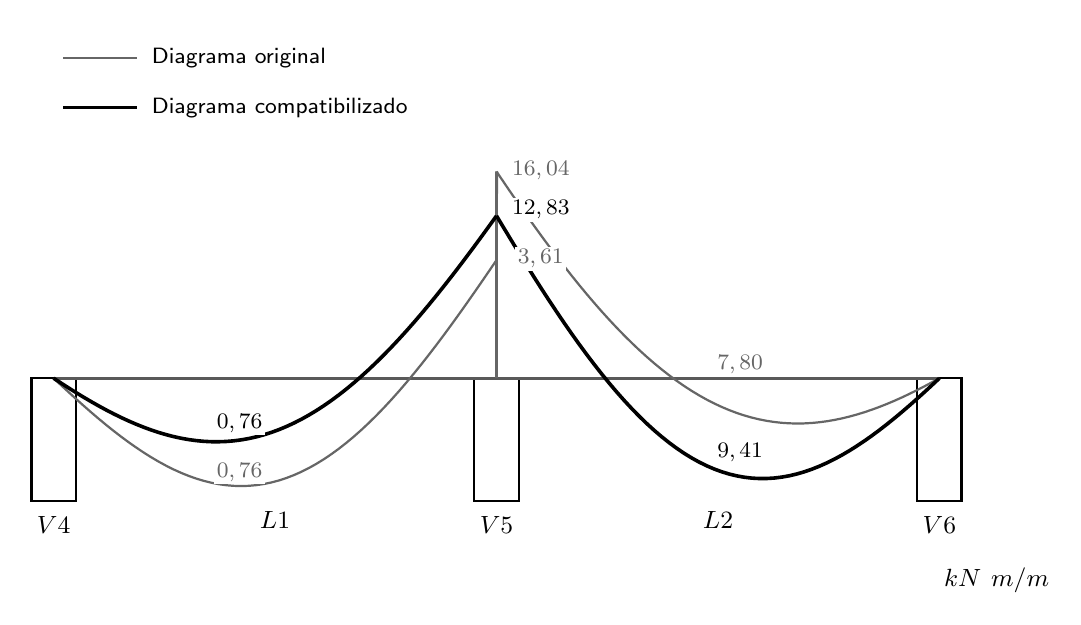
\begin{tikzpicture}[
        scale=1.25,
        pilar/.style={draw=black, thick, fill=white},
        viga/.style={line width=1pt, gray!70!black},
        linhaOriginal/.style={thick, gray!80!black},
        linhaCompat/.style={line width=1.3pt, black},
        cota/.style={<->, >=stealth, thin, black},
        chamada/.style={gray!50, thin, dashed}
    ]
    
        % --- Parâmetros de Geometria ---
        \def\L{4.5} % Comprimento de cada vão
    
        % Coordenadas dos Apoios/Pilares
        \coordinate (P1) at (0, 0);
        \coordinate (P2) at (\L, 0);
        \coordinate (P3) at (2*\L, 0);
    
        % 1. Desenho dos 3 Pilares (P1, P2, P3)
        \def\wP{0.45}
        \def\hP{1.25}
    
        % Pilar 1 (x = 0)
        \draw[pilar] (-\wP/2, -\hP) rectangle (\wP/2, 0);
        \node[below=2pt, font=\small\bfseries] at (0, -\hP) {$V4$};
    
        % Pilar 2 (x = L)
        \draw[pilar] (\L-\wP/2, -\hP) rectangle (\L+\wP/2, 0);
        \node[below=2pt, font=\small\bfseries] at (\L, -\hP) {$V5$};
    
        % Pilar 3 (x = 2L)
        \draw[pilar] (2*\L-\wP/2, -\hP) rectangle (2*\L+\wP/2, 0);
        \node[below=2pt, font=\small\bfseries] at (2*\L, -\hP) {$V6$};
    
        % Hachura sob a base dos pilares (Fundação)
        %\foreach \x in {0, \L, 2*\L} {
         %   \path[pattern={Lines[angle=45, distance=3pt, line width=0.4pt]}, pattern color=gray!60]
          %      (\x-\wP/2, -\hP-0.15) rectangle (\x+\wP/2, -\hP);
           % \draw[thick] (\x-\wP/2, -\hP) -- (\x+\wP/2, -\hP);
        %}
    
        % 2. Eixo das Vigas (V1 e V2)
        \draw[viga] (0, 0) -- (2*\L, 0);
    
        % Rótulos das Vigas no Centro de Cada Vão (Parte Inferior)
        \node[below=2pt, font=\small\bfseries, fill=white, inner sep=1.5pt] at (\L/2, -\hP) {$L1$};
        \node[below=2pt, font=\small\bfseries, fill=white, inner sep=1.5pt] at (1.5*\L, -\hP) {$L2$};
        
        \node[right, font=\small\bfseries, fill=white, inner sep=1.5pt] at (2*\L, -\hP-0.8) {$kN \ m/m$};

    % CHAMADA MEIO

    % --- C. LINHA VERTICAL SAINDO DO PILAR P2 CONECTANDO OS TRÊS PONTOS ---
    \coordinate (Pt1) at (\L, 1.2);   % Ponto do diagrama original V1
    \coordinate (Pt2) at (\L, 1.65);  % Ponto do diagrama compatibilizado
    \coordinate (Pt3) at (\L, 2.1);   % Ponto do diagrama original V2

    % Linha vertical contínua que sai do topo do pilar P2 (x=L, y=0) e conecta os 3 pontos
    \draw[line width=1pt, gray!80!black] (\L, 0) -- (Pt3);

    % 3. DIAGRAMA DE MOMENTOS FLETORES

    % --- A. Linha Original (Antes da Compatibilização) ---
    % Vão 1 (0 a L): Original fica ABAIXO da compatibilizada
    \draw[linhaOriginal] 
        plot[domain=0:\L, samples=60] (\x, {-1.35 * sin(\x * 180 / \L) + 1.2 * (\x/\L)^2});

    % Vão 2 (L a 2L): Original fica ACIMA da compatibilizada
    \draw[linhaOriginal] 
        plot[domain=\L:2*\L, samples=60] (\x, {-0.8 * sin((\x-\L) * 180 / \L) + 2.1 * ((2*\L-\x)/\L)^2});

    % --- B. Linha Compatibilizada (Após a Compatibilização) ---
    % Vão 1: Compatibilizada fica acima da original no meio do vão
    \draw[linhaCompat] 
        plot[domain=0:\L, samples=60] (\x, {-0.95 * sin(\x * 180 / \L) + 1.65 * (\x/\L)^2});

    % Vão 2: Compatibilizada fica abaixo da original no meio do vão
    \draw[linhaCompat] 
        plot[domain=\L:2*\L, samples=60] (\x, {-1.35 * sin((\x-\L) * 180 / \L) + 1.65 * ((\x-\L)/\L - 1)^2});

    % 4. RÓTULOS DOS MOMENTOS MÁXIMOS (LOCALIZADOS NOS PRÓPRIOS PONTOS, SEM SETAS)

    % Sobre o Pilar P2 (Momentos Negativos):
        \node[above=3pt, font=\sffamily\footnotesize\bfseries, gray!80!black, fill=white, inner sep=1pt] 
        at (\L+0.45, 1) {$3,61$};
    \node[above=3pt, font=\sffamily\footnotesize\bfseries, gray!80!black, fill=white, inner sep=1pt] 
        at (\L+0.45, 1.9) {$16,04$};

    \node[above=3pt, font=\sffamily\footnotesize\bfseries, black, fill=white, inner sep=1pt] 
        at (\L+0.45, 1.5) {$12,83$};

    % No Vão 1 (V1):
    \node[below=1pt, font=\sffamily\footnotesize\bfseries, gray!80!black, fill=white, inner sep=1pt] 
        at (0.42*\L, -0.8) {$0,76$};
    \node[below=1pt, font=\sffamily\footnotesize\bfseries, black, fill=white, inner sep=1pt] 
        at (0.42*\L, -0.3) {$0,76$};

    % No Vão 2 (V2) - Maior que no vão V1:
    \node[below=1pt, font=\sffamily\footnotesize\bfseries, gray!80!black, fill=white, inner sep=1pt] 
        at (1.55*\L, 0.3) {$7,80$};
    \node[below=1pt, font=\sffamily\footnotesize\bfseries, black, fill=white, inner sep=1pt] 
        at (1.55*\L, -0.6) {$9,41$};

    
        % 5. LEGENDA
        \begin{scope}[shift={(0, 3)}]
            \draw[thick, fill=white, draw=white] (-0.1, -0.55) rectangle (3.3, 0.55);
            \draw[linhaOriginal] (0.1, 0.25) -- (0.85, 0.25);
            \node[right, font=\sffamily\footnotesize] at (0.9, 0.25) {Diagrama original};
            \draw[linhaCompat] (0.1, -0.25) -- (0.85, -0.25);
            \node[right, font=\sffamily\footnotesize] at (0.9, -0.25) {Diagrama compatibilizado};
        \end{scope}
    \end{tikzpicture}
    
    %\caption{Caption}
    %label{fig:placeholder}
\end{figure}
    
                \begin{observacao}
                    Não precisa fazer a compatibilização da L1 para ficar a favor da segurança.
                \\ref{}end{observacao}
                \end{observacao}
    
                $M_{med} \geq \begin{cases}
                    \frac{M'+M'_{0}}{2} = \frac{16,04+3,61}{2}=9,83 \ kN m/m \\
                    0,8M'=0,8 \times 16,04 = 12,83 \ kN m/m
                \end{cases}$
    
                $M_{c,\ L2}= M_{eixo} + \frac{M'-M_{med}}{2}= 7,8 + \frac{16,04 - 12,83}{2} = 9,41 \ kN m/m$ \newline
                
                \item Corte BB

                \begin{figure}[H]
    \centering

    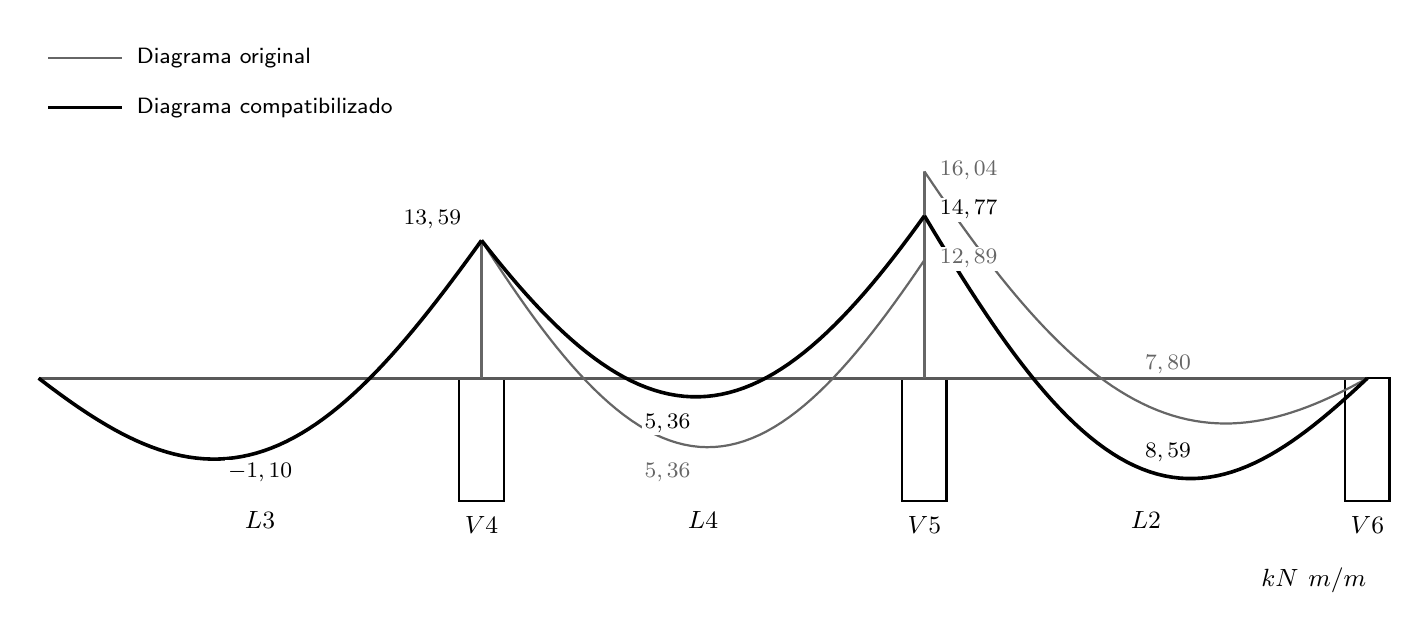
\begin{tikzpicture}[
        scale=1.25,
        pilar/.style={draw=black, thick, fill=white},
        viga/.style={line width=1pt, gray!70!black},
        linhaOriginal/.style={thick, gray!80!black},
        linhaCompat/.style={line width=1.3pt, black},
        cota/.style={<->, >=stealth, thin, black},
        chamada/.style={gray!50, thin, dashed}
    ]

        % --- Parâmetros de Geometria ---
        \def\L{4.5} % Comprimento de cada vão
        \def\Mneg{1.4} % Altura (desenho) do momento negativo em V4 (igual original/compat.)

        % Coordenadas dos Apoios/Pilares
        \coordinate (P0) at (-\L, 0);
        \coordinate (P1) at (0, 0);
        \coordinate (P2) at (\L, 0);
        \coordinate (P3) at (2*\L, 0);

        % 1. Desenho dos 4 Pilares
        \def\wP{0.45}
        \def\hP{1.25}

        % Pilar 0 (x = -L) -- NOVO
        %\draw[pilar] (-\L-\wP/2, -\hP) rectangle (-\L+\wP/2, 0);
        %\node[below=2pt, font=\small\bfseries] at (-\L, -\hP) {$V3$};

        % Pilar 1 (x = 0)
        \draw[pilar] (-\wP/2, -\hP) rectangle (\wP/2, 0);
        \node[below=2pt, font=\small\bfseries] at (0, -\hP) {$V4$};

        % Pilar 2 (x = L)
        \draw[pilar] (\L-\wP/2, -\hP) rectangle (\L+\wP/2, 0);
        \node[below=2pt, font=\small\bfseries] at (\L, -\hP) {$V5$};

        % Pilar 3 (x = 2L)
        \draw[pilar] (2*\L-\wP/2, -\hP) rectangle (2*\L+\wP/2, 0);
        \node[below=2pt, font=\small\bfseries] at (2*\L, -\hP) {$V6$};

        % 2. Eixo das Vigas (agora de -L a 2L)
        \draw[viga] (-\L, 0) -- (2*\L, 0);

        % Rótulos das Vigas no Centro de Cada Vão (Parte Inferior)
        \node[below=2pt, font=\small\bfseries, fill=white, inner sep=1.5pt] at (-\L/2, -\hP) {$L3$};
        \node[below=2pt, font=\small\bfseries, fill=white, inner sep=1.5pt] at (\L/2, -\hP) {$L4$};
        \node[below=2pt, font=\small\bfseries, fill=white, inner sep=1.5pt] at (1.5*\L, -\hP) {$L2$};

        \node[right, font=\small\bfseries, fill=white, inner sep=1.5pt] at (1.75*\L, -\hP-0.8) {$kN \ m/m$};

    % CHAMADA MEIO

    % --- C. LINHAS VERTICAIS NOS PILARES ---
    \coordinate (Pt1) at (\L, 1.2);   % Ponto do diagrama original V1
    \coordinate (Pt2) at (\L, 1.65);  % Ponto do diagrama compatibilizado
    \coordinate (Pt3) at (\L, 2.1);   % Ponto do diagrama original V2

    \draw[line width=1pt, gray!80!black] (\L, 0) -- (Pt3);

    % Linha vertical em V4 (momento negativo igual no original e no compatibilizado)
    \draw[line width=1pt, gray!80!black] (0, 0) -- (0, \Mneg);

    % 3. DIAGRAMA DE MOMENTOS FLETORES

    % --- NOVO VÃO L0 (-L a 0): original = compatibilizado ---
    \draw[linhaOriginal]
        plot[domain=-\L:0, samples=60] (\x, {-1.10 * sin((\x+\L) * 180 / \L) + \Mneg * ((\x+\L)/\L)^2});
    \draw[linhaCompat]
        plot[domain=-\L:0, samples=60] (\x, {-1.10 * sin((\x+\L) * 180 / \L) + \Mneg * ((\x+\L)/\L)^2});

    % --- A. Linha Original (Antes da Compatibilização) ---
    % Vão 1 (0 a L): agora com momento negativo também em x=0
    \draw[linhaOriginal]
        plot[domain=0:\L, samples=60] (\x, {-1.35 * sin(\x * 180 / \L) + 1.2 * (\x/\L)^2 + \Mneg * ((\L-\x)/\L)^2});

    % Vão 2 (L a 2L)
    \draw[linhaOriginal]
        plot[domain=\L:2*\L, samples=60] (\x, {-0.8 * sin((\x-\L) * 180 / \L) + 2.1 * ((2*\L-\x)/\L)^2});

    % --- B. Linha Compatibilizada (Após a Compatibilização) ---
    % Vão 1
    \draw[linhaCompat]
        plot[domain=0:\L, samples=60] (\x, {-0.95 * sin(\x * 180 / \L) + 1.65 * (\x/\L)^2 + \Mneg * ((\L-\x)/\L)^2});

    % Vão 2
    \draw[linhaCompat]
        plot[domain=\L:2*\L, samples=60] (\x, {-1.35 * sin((\x-\L) * 180 / \L) + 1.65 * ((\x-\L)/\L - 1)^2});

    % 4. RÓTULOS DOS MOMENTOS MÁXIMOS

    % Sobre o Pilar V4 (momento negativo, igual original/compat.) -- NOVO
    \node[above=3pt, font=\sffamily\footnotesize\bfseries, black, fill=white, inner sep=1pt]
        at (-0.5, \Mneg) {$13,59$};

    % No Vão L0 (igual original/compat.) -- NOVO
    \node[below=1pt, font=\sffamily\footnotesize\bfseries, black, fill=white, inner sep=1pt]
        at (-0.5*\L, -0.8) {$-1,10$};

    % Sobre o Pilar P2 (Momentos Negativos):
    \node[above=3pt, font=\sffamily\footnotesize\bfseries, gray!80!black, fill=white, inner sep=1pt]
        at (\L+0.45, 1) {$12,89$};
    \node[above=3pt, font=\sffamily\footnotesize\bfseries, gray!80!black, fill=white, inner sep=1pt]
        at (\L+0.45, 1.9) {$16,04$};

    \node[above=3pt, font=\sffamily\footnotesize\bfseries, black, fill=white, inner sep=1pt]
        at (\L+0.45, 1.5) {$14,77$};

    % No Vão 1 (V1):
    \node[below=1pt, font=\sffamily\footnotesize\bfseries, gray!80!black, fill=white, inner sep=1pt]
        at (0.42*\L, -0.8) {$5,36$};
    \node[below=1pt, font=\sffamily\footnotesize\bfseries, black, fill=white, inner sep=1pt]
        at (0.42*\L, -0.3) {$5,36$};

    % No Vão 2 (V2):
    \node[below=1pt, font=\sffamily\footnotesize\bfseries, gray!80!black, fill=white, inner sep=1pt]
        at (1.55*\L, 0.3) {$7,80$};
    \node[below=1pt, font=\sffamily\footnotesize\bfseries, black, fill=white, inner sep=1pt]
        at (1.55*\L, -0.6) {$8,59$};

        % 5. LEGENDA
        \begin{scope}[shift={(-\L, 3)}]
            \draw[thick, fill=white, draw=white] (-0.1, -0.55) rectangle (3.3, 0.55);
            \draw[linhaOriginal] (0.1, 0.25) -- (0.85, 0.25);
            \node[right, font=\sffamily\footnotesize] at (0.9, 0.25) {Diagrama original};
            \draw[linhaCompat] (0.1, -0.25) -- (0.85, -0.25);
            \node[right, font=\sffamily\footnotesize] at (0.9, -0.25) {Diagrama compatibilizado};
        \end{scope}
    \end{tikzpicture}

    %\caption{Caption}
    %label{fig:placeholder}
\end{figure}
    
                \begin{observacao}
                    Como a L3 é em balanço, os valores se mantém.
                \end{observacao}
    
                $M_{med} \geq \begin{cases}
                    \frac{M'+M'_{0}}{2} = \frac{16,04+12,89}{2}= 14,77 \ kN m/m \\
                    0,8M'=0,8 \times 16,04 = 12,83 \ kN m/m
                \end{cases}$
    
                $M_{c,\ L2}= M_{eixo} + \frac{M'-M_{med}}{2}= 7,8 + \frac{16,04 - 14,77}{2} = 8,59 \ kN m/m$ \newline
                
                \item Corte CC

                \begin{figure}[H]
    \centering

    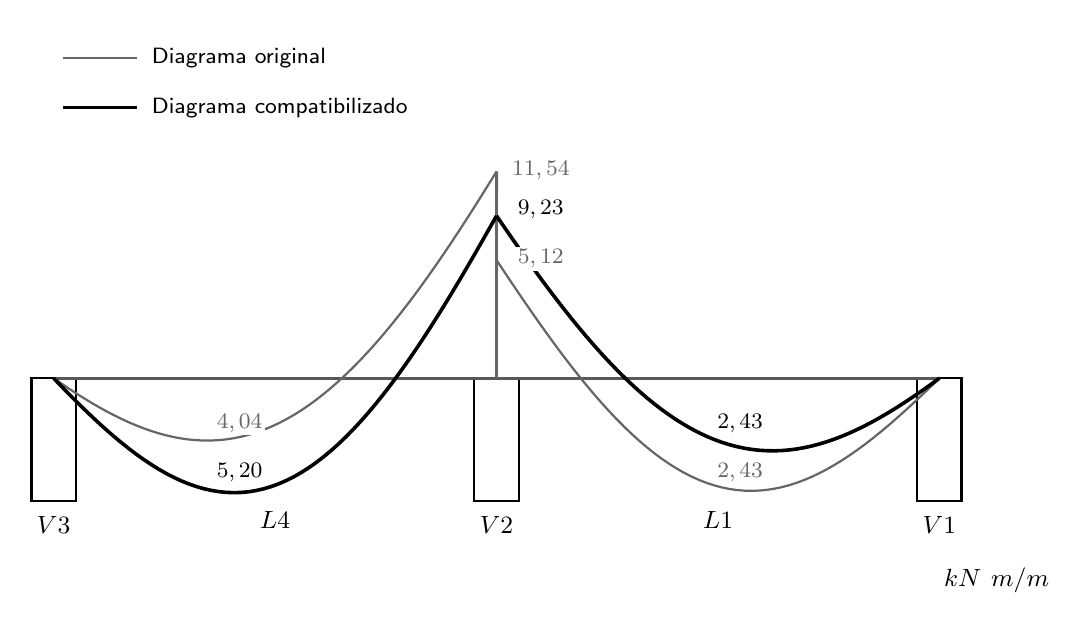
\begin{tikzpicture}[
        scale=1.25,
        pilar/.style={draw=black, thick, fill=white},
        viga/.style={line width=1pt, gray!70!black},
        linhaOriginal/.style={thick, gray!80!black},
        linhaCompat/.style={line width=1.3pt, black},
        cota/.style={<->, >=stealth, thin, black},
        chamada/.style={gray!50, thin, dashed}
    ]
    
        % --- Parâmetros de Geometria ---
        \def\L{4.5} % Comprimento de cada vão
    
        % Coordenadas dos Apoios/Pilares
        \coordinate (P1) at (0, 0);
        \coordinate (P2) at (\L, 0);
        \coordinate (P3) at (2*\L, 0);
    
        % 1. Desenho dos 3 Pilares (P1, P2, P3)
        \def\wP{0.45}
        \def\hP{1.25}
    
        % Pilar 1 (x = 0)
        \draw[pilar] (-\wP/2, -\hP) rectangle (\wP/2, 0);
        \node[below=2pt, font=\small\bfseries] at (0, -\hP) {$V3$};
    
        % Pilar 2 (x = L)
        \draw[pilar] (\L-\wP/2, -\hP) rectangle (\L+\wP/2, 0);
        \node[below=2pt, font=\small\bfseries] at (\L, -\hP) {$V2$};
    
        % Pilar 3 (x = 2L)
        \draw[pilar] (2*\L-\wP/2, -\hP) rectangle (2*\L+\wP/2, 0);
        \node[below=2pt, font=\small\bfseries] at (2*\L, -\hP) {$V1$};
    
        % Hachura sob a base dos pilares (Fundação)
        %\foreach \x in {0, \L, 2*\L} {
         %   \path[pattern={Lines[angle=45, distance=3pt, line width=0.4pt]}, pattern color=gray!60]
          %      (\x-\wP/2, -\hP-0.15) rectangle (\x+\wP/2, -\hP);
           % \draw[thick] (\x-\wP/2, -\hP) -- (\x+\wP/2, -\hP);
        %}
    
        % 2. Eixo das Vigas (V1 e V2)
        \draw[viga] (0, 0) -- (2*\L, 0);
    
        % Rótulos das Vigas no Centro de Cada Vão (Parte Inferior)
        \node[below=2pt, font=\small\bfseries, fill=white, inner sep=1.5pt] at (\L/2, -\hP) {$L4$};
        \node[below=2pt, font=\small\bfseries, fill=white, inner sep=1.5pt] at (1.5*\L, -\hP) {$L1$};
        
        \node[right, font=\small\bfseries, fill=white, inner sep=1.5pt] at (2*\L, -\hP-0.8) {$kN \ m/m$};

    % CHAMADA MEIO

    % --- C. LINHA VERTICAL SAINDO DO PILAR P2 CONECTANDO OS TRÊS PONTOS ---
    \coordinate (Pt1) at (\L, 1.2);   % Ponto do diagrama original V1
    \coordinate (Pt2) at (\L, 1.65);  % Ponto do diagrama compatibilizado
    \coordinate (Pt3) at (\L, 2.1);   % Ponto do diagrama original V2

    % Linha vertical contínua que sai do topo do pilar P2 (x=L, y=0) e conecta os 3 pontos
    \draw[line width=1pt, gray!80!black] (\L, 0) -- (Pt3);

    % 3. DIAGRAMA DE MOMENTOS FLETORES

    % --- A. Linha Original (Antes da Compatibilização) ---
    % Vão 1 (0 a L): Original fica ACIMA da compatibilizada (menos profunda)
    \draw[linhaOriginal] 
        plot[domain=0:\L, samples=60] (\x, {-1.0 * sin(\x * 180 / \L) + 2.1 * (\x/\L)^2});

    % Vão 2 (L a 2L): Original fica ABAIXO da compatibilizada (mais profunda)
    \draw[linhaOriginal] 
        plot[domain=\L:2*\L, samples=60] (\x, {-1.4 * sin((\x-\L) * 180 / \L) + 1.2 * ((2*\L-\x)/\L)^2});

    % --- B. Linha Compatibilizada (Após a Compatibilização) ---
    % Vão 1: Compatibilizada fica ABAIXO da original no meio do vão
    \draw[linhaCompat] 
        plot[domain=0:\L, samples=60] (\x, {-1.5 * sin(\x * 180 / \L) + 1.65 * (\x/\L)^2});

    % Vão 2: Compatibilizada fica ACIMA da original no meio do vão
    \draw[linhaCompat] 
        plot[domain=\L:2*\L, samples=60] (\x, {-1.05 * sin((\x-\L) * 180 / \L) + 1.65 * ((\x-\L)/\L - 1)^2});

    % 4. RÓTULOS DOS MOMENTOS MÁXIMOS (LOCALIZADOS NOS PRÓPRIOS PONTOS, SEM SETAS)

    % Sobre o Pilar P2 (Momentos Negativos):
        \node[above=3pt, font=\sffamily\footnotesize\bfseries, gray!80!black, fill=white, inner sep=1pt] 
        at (\L+0.45, 1) {$5,12$};
    \node[above=3pt, font=\sffamily\footnotesize\bfseries, gray!80!black, fill=white, inner sep=1pt] 
        at (\L+0.45, 1.9) {$11,54$};

    \node[above=3pt, font=\sffamily\footnotesize\bfseries, black, fill=white, inner sep=1pt] 
        at (\L+0.45, 1.5) {$9,23$};

    % No Vão 1 (V1):
    \node[below=1pt, font=\sffamily\footnotesize\bfseries, gray!80!black, fill=white, inner sep=1pt] 
        at (0.42*\L, -0.3) {$4,04$};
    \node[below=1pt, font=\sffamily\footnotesize\bfseries, black, fill=white, inner sep=1pt] 
        at (0.42*\L, -0.8) {$5,20$};

    % No Vão 2 (V2) - Maior que no vão V1:
    \node[below=1pt, font=\sffamily\footnotesize\bfseries, gray!80!black, fill=white, inner sep=1pt] 
        at (1.55*\L, -0.8) {$2,43$};
    \node[below=1pt, font=\sffamily\footnotesize\bfseries, black, fill=white, inner sep=1pt] 
        at (1.55*\L, -0.3) {$2,43$};

    
        % 5. LEGENDA
        \begin{scope}[shift={(0, 3)}]
            \draw[thick, fill=white, draw=white] (-0.1, -0.55) rectangle (3.3, 0.55);
            \draw[linhaOriginal] (0.1, 0.25) -- (0.85, 0.25);
            \node[right, font=\sffamily\footnotesize] at (0.9, 0.25) {Diagrama original};
            \draw[linhaCompat] (0.1, -0.25) -- (0.85, -0.25);
            \node[right, font=\sffamily\footnotesize] at (0.9, -0.25) {Diagrama compatibilizado};
        \end{scope}
    \end{tikzpicture}
    
    %\caption{Caption}
    %label{fig:placeholder}
\end{figure}
    
                \begin{observacao}
                    Não precisa fazer a compatibilização da L1 para ficar a favor da segurança.
                \end{observacao}
    
                $M_{med} \geq \begin{cases}
                    \frac{M'+M'_{0}}{2} = \frac{11,54+5,12}{2}=8,83 \ kN m/m \\
                    0,8M'=0,8 \times 11,54 = 9,23 \ kN m/m
                \end{cases}$
    
                $M_{c,\ L4}= M_{eixo} + \frac{M'-M_{med}}{2}= 4,04 + \frac{11,54 - 9,23}{2} = 5,20 \ kN m/m$ \newline
            \end{enumerate}
    
            \begin{figure}[H]
    \centering
    \begin{tikzpicture}[
        scale=1.5,
        retangulo/.style={draw=gray!80!black, thick},
        rotuloLetra/.style={font=\footnotesize, blue!80!black},
        eixo/.style={->, >=stealth, thick, black},
        corte/.style={draw=black, dash dot, thick},
        setaCorte/.style={->, >=stealth, thick, black}
    ]

        % --- Definição dos Parâmetros de Dimensão ---
        \def\wCentro{3.2}       % Largura dos retângulos centrais (L1 e L3)
        \def\hCima{2.0}         % Altura do retângulo superior (L1)
        \def\hBaixo{2.2}        % Altura do retângulo inferior (L3)
        
        \def\wDir{2.2}          % Largura do retângulo da direita (L2)
        \def\hDir{\hCima + \hBaixo} % Altura total da laje L2
        
        \def\wEsq{1.6}          % Largura do retângulo da esquerda (L4)
        \def\hEsq{\hBaixo}      % Altura da laje L4

        % --- Coordenadas ---
        \coordinate (A2) at (0, 0);
        \coordinate (B2) at (\wCentro, 0);
        \coordinate (C2) at (\wCentro, \hBaixo);
        \coordinate (D2) at (0, \hBaixo);

        \coordinate (A1) at (0, \hBaixo);
        \coordinate (B1) at (\wCentro, \hBaixo);
        \coordinate (C1) at (\wCentro, \hBaixo + \hCima);
        \coordinate (D1) at (0, \hBaixo + \hCima);

        \coordinate (A3) at (\wCentro, 0);
        \coordinate (B3) at (\wCentro + \wDir, 0);
        \coordinate (C3) at (\wCentro + \wDir, \hDir);
        \coordinate (D3) at (\wCentro, \hDir);

        \coordinate (A4) at (-\wEsq, 0);
        \coordinate (B4) at (0, 0);
        \coordinate (C4) at (0, \hEsq);
        \coordinate (D4) at (-\wEsq, \hEsq);

        % --- Desenho dos Retângulos ---
        \draw[retangulo] (A1) rectangle (C1); % L1
        \draw[retangulo] (A2) rectangle (C2); % L3
        \draw[retangulo] (A3) rectangle (C3); % L2
        \draw[retangulo] (A4) rectangle (C4); % L4

        % --- EIXOS LOCALIZADOS COM NÚMERO NO CENTRO DE CADA EIXO ---
        % L1 (Topo)
        \coordinate (CL1) at ($(A1)!0.4!(C1)$);
        \draw[eixo] (CL1) -- ($(CL1)+(0.55,0)$) 
            node[midway, below=2pt, blue!80!black, fill=white, inner sep=1pt, font=\footnotesize] {0,76} 
            node[right=-2pt, font=\small] {$y$};
        \draw[eixo] (CL1) -- ($(CL1)+(0,0.55)$) 
            node[midway, left=2pt, blue!80!black, fill=white, inner sep=1pt, font=\footnotesize] {2,43} 
            node[above=-2pt, font=\small] {$x$};

        % L3 (Baixo)
        \coordinate (CL3) at ($(A2)!0.4!(C2)$);
        \draw[eixo] (CL3) -- ($(CL3)+(0.55,0)$) 
            node[midway, below=2pt, blue!80!black, fill=white, inner sep=1pt, font=\footnotesize] {5,36} 
            node[right=-2pt, font=\small] {$x$};
        \draw[eixo] (CL3) -- ($(CL3)+(0,0.55)$) 
            node[midway, left=2pt, blue!80!black, fill=white, inner sep=1pt, font=\footnotesize] {4,04} 
            node[above=-2pt, font=\small] {$y$};

        % L4 (Esquerda)
        \coordinate (CL4) at ($(A4)!0.4!(C4)$);
        \draw[eixo] (CL4) -- ($(CL4)+(0.55,0)$) 
            node[midway, below=2pt, blue!80!black, fill=white, inner sep=1pt, font=\footnotesize] {-1,10} 
            node[right=-2pt, font=\small] {$x$};
        \draw[eixo] (CL4) -- ($(CL4)+(0,0.55)$) 
            node[midway, left=2pt, blue!80!black, fill=white, inner sep=1pt, font=\footnotesize] {0,07} 
            node[above=-2pt, font=\small] {$y$};

        % L2 - Eixo Superior (Alinhado em Y com L1)
        \coordinate (CL2_top) at (\wCentro + 0.4*\wDir, \hBaixo + 0.4*\hCima);
        \draw[eixo] (CL2_top) -- ($(CL2_top)+(0.55,0)$) 
            node[midway, below=2pt, blue!80!black, fill=white, inner sep=1pt, font=\footnotesize] {9,41} 
            node[right=-2pt, font=\small] {$x$};
        \draw[eixo] (CL2_top) -- ($(CL2_top)+(0,0.55)$) 
            node[midway, left=2pt, blue!80!black, fill=white, inner sep=1pt, font=\footnotesize] {2,24}
            node[above=-2pt, font=\small] {$y$};

        % L2 - Eixo Inferior (Alinhado em Y com L3 e L4 - Cotas 7,80 / 2,24)
        \coordinate (CL2_bot) at (\wCentro + 0.4*\wDir, 0.4*\hBaixo);
        \draw[eixo] (CL2_bot) -- ($(CL2_bot)+(0.55,0)$) 
            node[midway, below=2pt, blue!80!gray, fill=white, inner sep=1pt, font=\footnotesize] {8,59} 
            node[right=-2pt, font=\small] {$x$};
        \draw[eixo] (CL2_bot) -- ($(CL2_bot)+(0,0.55)$) 
            node[midway, left=2pt, blue!80!gray, fill=white, inner sep=1pt, font=\footnotesize] {2,24} 
            node[above=-2pt, font=\small] {$y$};


        % --- LINHAS DE CORTE A, B e C ---
        % Corte A: passa na L1 e L2
        %\draw[corte] (-0.4, 2.85) -- (\wCentro + \wDir + 0.4, 2.85);
        %\draw[setaCorte] (-0.4, 2.85) -- (-0.4, 3.15) node[above, font=\small\bfseries] {A};
        %\draw[setaCorte] (\wCentro + \wDir + 0.4, 2.85) -- (\wCentro + \wDir + 0.4, 3.15) node[above, font=\small\bfseries] {A};

        % Corte B: da L3 a L2 (passando por L4)
        %\draw[corte] (-\wEsq - 0.4, 0.5) -- (\wCentro + \wDir + 0.4, 0.5);
        %\draw[setaCorte] (-\wEsq - 0.4, 0.5) -- (-\wEsq - 0.4, 0.8) node[above, font=\small\bfseries] {B};
        %\draw[setaCorte] (\wCentro + \wDir + 0.4, 0.5) -- (\wCentro + \wDir + 0.4, 0.8) node[above, font=\small\bfseries] {B};

        % Corte C: de L1 a L4
        %\draw[corte] (0.6, \hDir + 0.4) -- (0.6, -0.4);
        %\draw[setaCorte] (0.6, \hDir + 0.4) -- (0.9, \hDir + 0.4) node[right, font=\small\bfseries] {C};
        %\draw[setaCorte] (0.6, -0.4) -- (0.9, -0.4) node[right, font=\small\bfseries] {C};

        % --- Rótulos de Esforço Cortante nas Arestas ---
        % L1 (Topo)
        %\node[below, rotuloLetra] at ($(D1)!0.5!(C1)$) {$V_x$}; 
        %\node[right, rotuloLetra] at ($(D1)!0.5!(A1)$) {$V_y$}; 
        \node[ rotuloLetra, fill=white, inner sep=1pt] at ($(A1)!0.5!(B1)$) {9,23};
        \node[rotuloLetra, fill=white, inner sep=1pt]  at ($(B1)!0.5!(C1)$) {12,83}; 

        % L3 (Baixo)
        %\node[below, rotuloLetra] at ($(A1)!0.5!(B1)$) {$11,54$};
        %\node[right, rotuloLetra] at ($(D2)!0.5!(A2)$) {$0$}; 
        %\node[above, rotuloLetra] at ($(A2)!0.5!(B2)$) {$V_y$};
        \node[rotuloLetra, fill=white, inner sep=1pt]  at ($(B2)!0.5!(C2)$) {14,77};  
        
        % L2 (Direita)
        %\node[right, rotuloLetra] at ($(B1)!0.5!(C2)$) {$16,04$}; 
        %\node[below, rotuloLetra] at ($(D3)!0.5!(C3)$) {$V_y$}; 
        %\node[left= rotuloLetra]  at ($(C3)!0.5!(B3)$) {$V_x$}; 
        %\node[above, rotuloLetra] at ($(A3)!0.5!(B3)$) {$V_y$}; 

        % L4 (Esquerda)
        \node[rotuloLetra, fill=white, inner sep=1pt]  at ($(D2)!0.5!(A2)$) {13,59}; 
        %\node[below, rotuloLetra] at ($(D4)!0.5!(C4)$) {$V_y$}; 
        %\node[above, rotuloLetra] at ($(A4)!0.5!(B4)$) {$V_y$}; 
        \node[left, rotuloLetra]  at ($(D4)!0.5!(A4)$) {0,98}; 
        \draw[retangulo,white,dashed] (D4) rectangle (A4);
        
        \node[below, right=50pt] at ($(A3)!0.5!(B3)$) {$kN m/m$}; 

    \end{tikzpicture}
    %\caption{Arranjo de lajes com eixos locais numerados e cortes transversais A, B e C}
    %\label{fig:lajes_cortes}
\end{figure}

        \item Método ABNT
    
            \begin{figure}[H]
    \centering
    \begin{tikzpicture}[
        scale=1.5,
        retangulo/.style={draw=gray!80!black, thick},
        rotuloLetra/.style={font=\footnotesize, blue!80!black},
        eixo/.style={->, >=stealth, thick, black},
        corte/.style={draw=black, dash dot, thick},
        setaCorte/.style={->, >=stealth, thick, black}
    ]

        % --- Definição dos Parâmetros de Dimensão ---
        \def\wCentro{3.2}       % Largura dos retângulos centrais (L1 e L3)
        \def\hCima{2.0}         % Altura do retângulo superior (L1)
        \def\hBaixo{2.2}        % Altura do retângulo inferior (L3)
        
        \def\wDir{2.2}          % Largura do retângulo da direita (L2)
        \def\hDir{\hCima + \hBaixo} % Altura total da laje L2
        
        \def\wEsq{1.6}          % Largura do retângulo da esquerda (L4)
        \def\hEsq{\hBaixo}      % Altura da laje L4

        % --- Coordenadas ---
        \coordinate (A2) at (0, 0);
        \coordinate (B2) at (\wCentro, 0);
        \coordinate (C2) at (\wCentro, \hBaixo);
        \coordinate (D2) at (0, \hBaixo);

        \coordinate (A1) at (0, \hBaixo);
        \coordinate (B1) at (\wCentro, \hBaixo);
        \coordinate (C1) at (\wCentro, \hBaixo + \hCima);
        \coordinate (D1) at (0, \hBaixo + \hCima);

        \coordinate (A3) at (\wCentro, 0);
        \coordinate (B3) at (\wCentro + \wDir, 0);
        \coordinate (C3) at (\wCentro + \wDir, \hDir);
        \coordinate (D3) at (\wCentro, \hDir);

        \coordinate (A4) at (-\wEsq, 0);
        \coordinate (B4) at (0, 0);
        \coordinate (C4) at (0, \hEsq);
        \coordinate (D4) at (-\wEsq, \hEsq);

        % --- Desenho dos Retângulos ---
        \draw[retangulo] (A1) rectangle (C1); % L1
        \draw[retangulo] (A2) rectangle (C2); % L3
        \draw[retangulo] (A3) rectangle (C3); % L2
        \draw[retangulo] (A4) rectangle (C4); % L4

        % --- EIXOS LOCALIZADOS COM NÚMERO NO CENTRO DE CADA EIXO ---
        % L1 (Topo)
        \coordinate (CL1) at ($(A1)!0.4!(C1)$);
        \draw[eixo] (CL1) -- ($(CL1)+(0.55,0)$) 
            node[midway, below=2pt, blue!80!black, fill=white, inner sep=1pt, font=\footnotesize] {0,76} 
            node[right=-2pt, font=\small] {$y$};
        \draw[eixo] (CL1) -- ($(CL1)+(0,0.55)$) 
            node[midway, left=2pt, blue!80!black, fill=white, inner sep=1pt, font=\footnotesize] {2,43} 
            node[above=-2pt, font=\small] {$x$};

        % L3 (Baixo)
        \coordinate (CL3) at ($(A2)!0.4!(C2)$);
        \draw[eixo] (CL3) -- ($(CL3)+(0.55,0)$) 
            node[midway, below=2pt, blue!80!black, fill=white, inner sep=1pt, font=\footnotesize] {5,36} 
            node[right=-2pt, font=\small] {$x$};
        \draw[eixo] (CL3) -- ($(CL3)+(0,0.55)$) 
            node[midway, left=2pt, blue!80!black, fill=white, inner sep=1pt, font=\footnotesize] {4,04} 
            node[above=-2pt, font=\small] {$y$};

        % L4 (Esquerda)
        \coordinate (CL4) at ($(A4)!0.4!(C4)$);
        \draw[eixo] (CL4) -- ($(CL4)+(0.55,0)$) 
            node[midway, below=2pt, blue!80!black, fill=white, inner sep=1pt, font=\footnotesize] {-1,10} 
            node[right=-2pt, font=\small] {$x$};
        \draw[eixo] (CL4) -- ($(CL4)+(0,0.55)$) 
            node[midway, left=2pt, blue!80!black, fill=white, inner sep=1pt, font=\footnotesize] {0,07} 
            node[above=-2pt, font=\small] {$y$};

        % L2 
        \coordinate (CL2) at ($(A3)!0.5!(C3)$);
        \draw[eixo] (CL2) -- ($(CL2)+(0.55,0)$) 
            node[midway, below=2pt, blue!80!gray, fill=white, inner sep=1pt, font=\footnotesize] {7,80} 
            node[right=-2pt, font=\small] {$x$};
        \draw[eixo] (CL2) -- ($(CL2)+(0,0.55)$) 
            node[midway, left=2pt, blue!80!gray, fill=white, inner sep=1pt, font=\footnotesize] {2,24} 
            node[above=-2pt, font=\small] {$y$};


        % --- LINHAS DE CORTE A, B e C ---
        % Corte A: passa na L1 e L2
        %\draw[corte] (-0.4, 2.85) -- (\wCentro + \wDir + 0.4, 2.85);
        %\draw[setaCorte] (-0.4, 2.85) -- (-0.4, 3.15) node[above, font=\small\bfseries] {A};
        %\draw[setaCorte] (\wCentro + \wDir + 0.4, 2.85) -- (\wCentro + \wDir + 0.4, 3.15) node[above, font=\small\bfseries] {A};

        % Corte B: da L3 a L2 (passando por L4)
        %\draw[corte] (-\wEsq - 0.4, 0.5) -- (\wCentro + \wDir + 0.4, 0.5);
        %\draw[setaCorte] (-\wEsq - 0.4, 0.5) -- (-\wEsq - 0.4, 0.8) node[above, font=\small\bfseries] {B};
        %\draw[setaCorte] (\wCentro + \wDir + 0.4, 0.5) -- (\wCentro + \wDir + 0.4, 0.8) node[above, font=\small\bfseries] {B};

        % Corte C: de L1 a L4
        %\draw[corte] (0.6, \hDir + 0.4) -- (0.6, -0.4);
        %\draw[setaCorte] (0.6, \hDir + 0.4) -- (0.9, \hDir + 0.4) node[right, font=\small\bfseries] {C};
        %\draw[setaCorte] (0.6, -0.4) -- (0.9, -0.4) node[right, font=\small\bfseries] {C};

        % --- Rótulos de Esforço Cortante nas Arestas ---
        % L1 (Topo)
        %\node[below, rotuloLetra] at ($(D1)!0.5!(C1)$) {$V_x$}; 
        %\node[right, rotuloLetra] at ($(D1)!0.5!(A1)$) {$V_y$}; 
        \node[ rotuloLetra, fill=white, inner sep=1pt] at ($(A1)!0.5!(B1)$) {11,54};
        \node[rotuloLetra, fill=white, inner sep=1pt]  at ($(B1)!0.5!(C2)$) {16,04}; 

        % L3 (Baixo)
        %\node[below, rotuloLetra] at ($(A1)!0.5!(B1)$) {$11,54$};
        %\node[right, rotuloLetra] at ($(D2)!0.5!(A2)$) {$0$}; 
        %\node[above, rotuloLetra] at ($(A2)!0.5!(B2)$) {$V_y$};
        %\node[rotuloLetra, fill=white, inner sep=1pt]  at ($(B2)!0.5!(C2)$) {14,77};  
        
        % L2 (Direita)
        %\node[right, rotuloLetra] at ($(B1)!0.5!(C2)$) {$16,04$}; 
        %\node[below, rotuloLetra] at ($(D3)!0.5!(C3)$) {$V_y$}; 
        %\node[left= rotuloLetra]  at ($(C3)!0.5!(B3)$) {$V_x$}; 
        %\node[above, rotuloLetra] at ($(A3)!0.5!(B3)$) {$V_y$}; 

        % L4 (Esquerda)
        \node[rotuloLetra, fill=white, inner sep=1pt]  at ($(D2)!0.5!(A2)$) {13,59}; 
        %\node[below, rotuloLetra] at ($(D4)!0.5!(C4)$) {$V_y$}; 
        %\node[above, rotuloLetra] at ($(A4)!0.5!(B4)$) {$V_y$}; 
        \node[left, rotuloLetra]  at ($(D4)!0.5!(A4)$) {0,98}; 
        \draw[retangulo,white,dashed] (D4) rectangle (A4);
        
        \node[below, right=50pt] at ($(A3)!0.5!(B3)$) {$kN m/m$}; 

    \end{tikzpicture}
    %\caption{Arranjo de lajes com eixos locais numerados e cortes transversais A, B e C}
    %\label{fig:lajes_cortes}
\end{figure}
            
        \end{enumerate}

        \newpage

        \section*{Dimensionamento a flexão por tabelas Kc e Ks}

        \begin{figure}[H]
    \centering
    \begin{tikzpicture}[
    scale=1,
    cota/.style={<->, >=stealth, thin, black},
    chamada/.style={gray!50, thin, dashed},
    deformacao/.style={line width=1.3pt, gray!80!black},
    tensao/.style={line width=1.3pt, red!80!black, fill=red!10},
    eixo/.style={dash dot, thin, gray!70!black},
    armadura/.style={draw=black, fill=black}
]

    % --- Parâmetros Geométricos ---
    \def\bw{2}           % Largura bw
    \def\h{4.0}          % Altura h
    \def\xn{2.0}         % Posição da linha neutra x
    \def\yAs{0.4}        % Centro de As (tração)
    \def\dl{0.45}        % d' (cobrimento até centro de A's)
    \def\eCu{0.9}        % Escala gráfica de epsilon_cu
    \def\gap{1.5}        % Distância entre diagramas

    % --- Valores derivados (calculados numericamente) ---
    \pgfmathsetmacro{\d}{\h-\yAs}                  % Altura útil d
    \pgfmathsetmacro{\yLN}{\h-\xn}                 % Cota Y da Linha Neutra
    \pgfmathsetmacro{\yAsl}{\h-\dl}                % Cota Y de A's
    \pgfmathsetmacro{\yBloco}{\h-0.8*\xn}          % Base do bloco y = 0,8x
    \pgfmathsetmacro{\yRcd}{\h-0.4*\xn}            % Posição de Rcd
    \pgfmathsetmacro{\eS}{\eCu*(\yLN-\yAs)/\xn}    % Escala gráfica de epsilon_s (compatível com a L.N.)
    \pgfmathsetmacro{\eSl}{\eCu*(\yAsl-\yLN)/\xn}  % Escala gráfica de epsilon_s' (compressão, para a esquerda)

    % Localização X de cada diagrama
    \def\xSec{0}
    \pgfmathsetmacro{\xDef}{\bw + \gap}
    \pgfmathsetmacro{\xTen}{\xDef + 2.2 + \gap}

    % ==========================================
    % 1. SEÇÃO TRANSVERSAL DE CONCRETO ARMADO
    % ==========================================
    \draw[thick, fill=white] (\xSec, 0) rectangle (\xSec + \bw, \h);

    % Armadura As (tração, inferior)
    \coordinate (As1) at (\xSec + 0.6, \yAs);
    \coordinate (As2) at (\xSec + \bw - 0.6, \yAs);
    \draw[armadura] (As1) circle (0.12);
    \draw[armadura] (As2) circle (0.12);
    \node[above=3pt, font=\small\bfseries] at ($(As1)!0.5!(As2)$) {$A_s$};

    % Armadura A's (compressão, superior)
    \coordinate (Asl1) at (\xSec + 0.6, \yAsl);
    \coordinate (Asl2) at (\xSec + \bw - 0.6, \yAsl);
    \draw[armadura] (Asl1) circle (0.12);
    \draw[armadura] (Asl2) circle (0.12);
    \node[below=3pt, font=\small\bfseries] at ($(Asl1)!0.5!(Asl2)$) {$A'_s$};

    % Estribo
    \draw[thick, rounded corners=2pt] (\xSec + 0.25, 0.25) rectangle (\xSec + \bw - 0.25, \h - 0.25);

    % Momento fletor de cálculo M_d (seta curva)
    \draw[->, >=stealth, line width=1.4pt]
        ({\xSec+\bw+0.5*cos(-55)}, {0.9+0.5*sin(-55)})
        arc[start angle=-55, end angle=55, radius=0.5];
    \node[right=1pt, font=\small\bfseries] at (\xSec+\bw+0.5, 0.9) {$M_d$};

    % ==========================================
    % 2. DIAGRAMA DE DEFORMAÇÕES (\epsilon)
    % ==========================================
    % Eixo de Referência
    \draw[thick] (\xDef, 0) -- (\xDef, \h);

    % Linha Neutra
    \draw[eixo] (\xSec - 0.2, \yLN) -- (\xTen + 3.6, \yLN) node[right, font=\footnotesize\bfseries] {L.N.};

    % Linha de Deformação
    \draw[deformacao] (\xDef - \eCu, \h) -- (\xDef + \eS, \yAs);

    % Preenchimento Suave
    %\fill[gray!10, opacity=0.5] (\xDef, \h) -- (\xDef - \eCu, \h) -- (\xDef, \yLN) -- cycle;
    %\fill[gray!10, opacity=0.5] (\xDef, \yLN) -- (\xDef + \eS, \yAs) -- (\xDef, \yAs) -- cycle;

    % Deformação no concreto (\epsilon_cu)
    \draw[->, >=stealth, thick, gray!80!black] (\xDef, \h) -- (\xDef - \eCu, \h);
    \node[above=2pt, font=\small\bfseries, gray!80!black] at (\xDef - 0.7, \h) {$\varepsilon_{cu}$};

    % Deformação na armadura comprimida (\epsilon'_s)
    \draw[->, >=stealth, thick, gray!80!black] (\xDef, \yAsl) -- (\xDef - \eSl, \yAsl);
    \node[right=3pt, font=\small\bfseries, gray!80!black] at (\xDef, \yAsl) {$\varepsilon'_s$};

    % Deformação na armadura tracionada (\epsilon_s)
    \draw[->, >=stealth, thick, gray!80!black] (\xDef, \yAs) -- (\xDef + \eS, \yAs)
        node[right=2pt, font=\small\bfseries, gray!80!black] {$\varepsilon_s$};

    \node[below=22pt, font=\small\bfseries] at (\xDef, 0) {ELU};

    % ==========================================
    % 3. DIAGRAMA DE TENSÕES SIMPLIFICADO (NBR 6118)
    % ==========================================
    % Eixo de Referência
    \draw[thick] (\xTen, 0) -- (\xTen, \h);

    % Bloco Retangular Simplificado (Profundidade y = 0,8 x)
    \fill[red!15] (\xTen, \h) rectangle (\xTen + 1.6, \yBloco);
    \draw[tensao] (\xTen, \h) -- (\xTen + 1.6, \h) -- (\xTen + 1.6, \yBloco) -- (\xTen, \yBloco);

    % Força de compressão do concreto Rcd
    \draw[->, >=stealth, line width=1.5pt, black] (\xTen + 2.3, \yRcd) -- (\xTen + 0.1, \yRcd)
        node[pos=0, right=2pt, font=\small\bfseries] {$R_{cd}$};

    % Força de compressão da armadura R's
    \draw[->, >=stealth, line width=1.5pt, black] (\xTen + 2.3, \yAsl) -- (\xTen + 0.1, \yAsl)
        node[pos=0, right=2pt, font=\small\bfseries] {$R'_s$};

    % Força de tração da armadura Rs
    \draw[->, >=stealth, line width=1.5pt, black] (\xTen, \yAs) -- (\xTen + 2.2, \yAs)
        node[pos=1, right=2pt, font=\small\bfseries] {$R_s$};

    % Tensão no concreto
    \node[above=2pt, font=\small\bfseries, black] at (\xTen + 0.8, \h) {$\sigma_{cd}$};

    \node[below=22pt, font=\small\bfseries] at (\xTen + 0.8, 0) {Tensões};

    % ==========================================
    % 4. COTAS DE DIMENSÃO
    % ==========================================
    \def\offLeft{1.2}

    % Base bw
    \draw[cota] (\xSec, -0.4) -- (\xSec + \bw, -0.4)
        node[midway, fill=white, inner sep=1.5pt, font=\small\bfseries] {$b_w$};

    % Altura x (Linha Neutra)
    \draw[chamada] (\xDef, \h) -- (\xDef - \offLeft, \h);
    \draw[chamada] (\xDef, \yLN) -- (\xDef - \offLeft, \yLN);
    \draw[cota] (\xDef - \offLeft + 0.1, \yLN) -- (\xDef - \offLeft + 0.1, \h)
        node[midway, left=1pt, font=\small\bfseries] {$x$};

    % Altura do Bloco y = 0,8 x
    %\draw[chamada] (\xTen + 1.6, \yBloco) -- (\xTen + 3.4, \yBloco);
    %\draw[chamada] (\xTen + 1.6, \h) -- (\xTen + 3.4, \h);
    \draw[cota] (\xTen + 3.3, \yBloco) -- (\xTen + 3.3, \h)
        node[midway, right=1pt, font=\small\bfseries] {$y = \lambda\ x$};

    % Braço de alavanca z (entre Rcd e Rs)
    \draw[chamada] (\xTen, \yRcd) -- (\xTen - 0.5, \yRcd);
    \draw[chamada] (\xTen, \yAs) -- (\xTen - 0.5, \yAs);
    \draw[cota] (\xTen - 0.4, \yAs) -- (\xTen - 0.4, \yRcd)
        node[midway, left=1pt, font=\small\bfseries] {$z$};

    % Altura útil d
    \draw[cota] (\xSec - 0.8, \yAs) -- (\xSec - 0.8, \h)
        node[midway, left=1pt, font=\small\bfseries] {$d$};

    % Altura total h
    \draw[cota] (\xSec - 1.4, 0) -- (\xSec - 1.4, \h)
        node[midway, left=1pt, font=\small\bfseries] {$h$};

    % Cobrimento d'
    \draw[cota] (\xSec - 0.35, \yAsl) -- (\xSec - 0.35, \h)
        node[midway, left=1pt, font=\scriptsize\bfseries] {$d'$};

    \end{tikzpicture}
    %\caption{dfdf}
    %\label{sfdf}
\end{figure}

        \subsection*{Equilíbrio de momento}

        $M_d = R_c \Big(d-\frac{y}{2}\Big)+R's(d-d')) \newline M_d = (b_w \ y \ \sigma_{cd})\Big(d-\frac{y}{2}\Big) + (A's \ \sigma'_s)(d-d') \newline M_d = (b_w \ \lambda \ x \ \alpha_c \ \eta_c \ f_{cd})\Big(d-\frac{\lambda \ x}{2}\Big) + (A's \ \sigma'_s)(d-d') \to \beta_x=\frac{x}{d} \leftrightarrow x = \beta_x \ d \newline M_d = b_w \ \lambda \ \beta_x \ d \ \alpha_c \ \eta_c \ f_{cd}\Big(d-\frac{\lambda \ \beta_x \ d}{2}\Big) + \cancelto{0}{(A's \ \sigma'_s)(d-d')} \newline M_d = b_w \ \lambda \ \beta_x \ d^2 \ \alpha_c \ \eta_c \ f_{cd}\Big(1-\frac{\lambda \beta_x}{2}\Big)$ \newline

        $\to f_{ck} = 40 \ MPa \ (\lambda = 0,8, \eta_c=1, \alpha_c=0,85)$

        $M_d = b_w \ \lambda \ \beta_x \ d^2 \ \alpha_c \ \eta_c \ f_{cd}\Big(1-\frac{\lambda \beta_x}{2}\Big) \newline M_d = 0,68 \ b_w \ d^2 \ f_{cd} \ \beta_x(1-0,4 \beta_x) \longleftrightarrow \cancelto{K_c=f(\beta_x,f_{cd})}{\frac{b_w \ d^2}{M_d}}=\frac{1}{0,68 \ \beta_x \ f_{cd} (1-0,4 \beta_x)}$ \newline

        \subsection*{Do equilíbrio de tensões}

        $M_d = R_s \Big(d-\frac{y}{2}\Big) \newline M_d = A_s \ \sigma_{sd} \Big(d-\frac{\lambda \ x}{2}\Big) \to \beta_x = \frac{x}{d} \leftrightarrow x = \beta_x \ d \newline M_d = A_s \ \sigma_{sd} \Big(d-\frac{\lambda \ \beta_x \ d}{2}\Big)$ \newline

        $\to f_{ck} < 50 \ MPa (\lambda = 0,80)$

        $M_d = A_s \ \sigma_{sd} \Big(d-\frac{\lambda \ \beta_x \ d}{2}\Big) \newline M_d = A_s \ \sigma_{sd} \ d\Big(1-0,4 \ \beta_x\Big) \newline \cancelto{K_s=f(\sigma_s,\beta_x)}{\frac{A_s \ \sigma_{sd}}{M_d}}=\frac{1}{1-0,4 \ \beta_x}$
    \end{enumerate}
\end{resposta}

\newpage

\section*{Exemplo}

\begin{enumerate}
    \item Calcule a área de aço. Dados: C25, aço CA-50, CAA-II.

    \begin{figure}[H]
    \centering
    \begin{tikzpicture}[
        scale=1,
        cota/.style={<->, >=stealth, thin, gray!80!black},
        chamada/.style={gray!60, thin, dashed},
        setaMomento/.style={->, >=stealth, line width=1.2pt, black},
        armadura/.style={draw=black, fill=black},
        estribo/.style={draw=black, line width=1.2pt, rounded corners=3pt}
    ]

        % --- Parâmetros ---
        \def\bw{2.8}        % Largura da base (bw)
        \def\h{4.2}         % Altura total (h)
        \def\cob{0.35}      % Espessura do cobrimento (c)

        % Coordenadas dos cantos da seção transversal
        \coordinate (A) at (0, 0);
        \coordinate (B) at (\bw, 0);
        \coordinate (C) at (\bw, \h);
        \coordinate (D) at (0, \h);

        % 1. Seção Transversal Retangular Externa
        \draw[thick, fill=white] (A) rectangle (C);

        % 2. Estribo (Retângulo interno com cantos arredondados)
        \draw[estribo] (\cob, \cob) rectangle (\bw - \cob, \h - \cob);

        % 3. Barras de Armadura de Tração As (Inferior)
        \def\yBarra{\cob + 0.22}
        \coordinate (As1) at (\cob + 0.3, \yBarra);
        \coordinate (As2) at (\bw - \cob - 0.3, \yBarra);

        \draw[armadura] (As1) circle (0.1);
        \draw[armadura] (As2) circle (0.1);

        % Rótulo da Armadura As
        \node[above, font=\small] at ($(As1)!0.5!(As2)$) {$A_s$};

        % Indicação/Rótulo do Estribo
        %\draw[->, >=stealth, thin, gray!80!black] (\bw/2 + 0.7, \h - \cob - 0.6) -- (\bw - \cob, \h - \cob - 0.6)
            %node[left=18pt, font=\small] {Estribo};

        % 4. Momento Fletor Aplicado Md (Seta Curva)
        \draw[setaMomento] (\bw + 2.9, \h/2 + 0.2) arc (90:-90:0.5)
            node[midway, left=2pt, font=\small] {$M_r = 120 \ kNm$};

        % 5. Cotas de Dimensão (bw, h, d, c)
        \def\offsetB{0.4}
        \def\offsetH{0.4}
        \def\offsetD{1.1}

        % Cota da Base bw
        %\draw[chamada] (A) -- (0, -\offsetB - 0.05);
        %\draw[chamada] (B) -- (\bw, -\offsetB - 0.05);
        \draw[cota] (0, -\offsetB) -- (\bw, -\offsetB)
            node[midway, below=2pt, font=\small\bfseries] {$b_w = 30 \ cm$};

        % Cota da Altura Total h (Esquerda)
        %\draw[chamada] (D) -- (-\offsetH - 0.05, \h);
        %\draw[chamada] (A) -- (-\offsetH - 0.05, 0);
        \draw[cota] (0 -\offsetD, 0) -- (0 -\offsetD, \h)
            node[midway, left=2pt, font=\small\bfseries] {$h= 45 \ cm$};

        % Cota da Altura Útil d (Direita)
        %\draw[chamada] (C) -- (\bw + \offsetD + 0.05, \h);
        %\draw[chamada] (\bw, \yBarra) -- (\bw + \offsetD + 0.05, \yBarra);
        \draw[cota] (0 -\offsetB, \yBarra) -- (0 -\offsetB, \h)
            node[midway, left=2pt, font=\small\bfseries] {$d$};

        % Linha de centro para indicação da altura útil d
        %\draw[dash dot, thin, gray!80!black] (0.2, \yBarra) -- (\bw + \offsetD + 0.05, \yBarra);

        % Cota do Cobrimento c (Inferior e Lateral)
        %\draw[chamada] (0, 0) -- (0, -\offsetB - 0.6);
        %\draw[chamada] (\cob, 0) -- (\cob, -\offsetB - 0.6);
        %\draw[cota] (0, -\offsetB - 0.45) -- (\cob, -\offsetB - 0.45)
            %node[midway, below=1pt, font=\footnotesize\bfseries] {$c$};

    \end{tikzpicture}
    %\caption{Seção transversal retangular com indicação do estribo, cobrimento $c$ e armadura $A_s$}
    %\label{fig:secao_cobrimento_estribo}
\end{figure}

    \begin{resposta}
        \begin{enumerate}
            \item Momento de projeto

            $\gamma_c = 1,4$ \cite[tabela 12.1]{nbr6118} \newline

            $M_d = \gamma_c \ M_r = 1,4 \times 120 = 168 \ kNm = 16\ 800\ kN \ cm$  \newline
            
            \item Altura útil

            $d = h - c - \phi_e - n\frac{\phi_\ell}{2} = 45 \cdot 10^{-2} - 25 \cdot 10^{-3} - 5 \cdot 10^{-3} - 2\ \frac{10 \cdot 10^{-3}}{2} = 41 \ cm$ \newline
            
            \item Kc

            $K_c = \frac{b_w \ d^2}{M_d} = \frac{30 \times 41^2}{16800} = 3 \ cm^2/kN$ \newline
            
            \item Tipo de armadura

            $\beta_x = 0,32 \leq 0,45 \to$ armadura simples, domínio 3 \cite[tabela 1.1a]{tabelaskcks} \newline
            
            \item Ks

            $K_s = 0,026$ \cite[tabela 1.1a]{tabelaskcks} \newline

            \item Área de aço

            $K_s = \frac{A_s \ d }{M_d} \longleftrightarrow A_s = \frac{K_s \ M_d}{d} = \frac{0,026 \times 16 800}{41} = 10,65 \ cm^2$
            
        \end{enumerate}
    \end{resposta}
\end{enumerate}